% Created 2021-12-15 Wed 17:18
\documentclass[9pt, b5paper]{article}
\usepackage[UTF8]{ctex}
\usepackage{xltxtra}
\usepackage{bera}
\usepackage[T1]{fontenc}
\usepackage[scaled]{beraserif}
\usepackage[scaled]{berasans}
\usepackage[scaled]{beramono}
\usepackage{graphicx}
\usepackage{xcolor}
\usepackage{multirow}
\usepackage{multicol}
\usepackage{float}
\usepackage{textcomp}
\usepackage{geometry}
\geometry{left=1.2cm,right=1.2cm,top=1.5cm,bottom=1.2cm}
\usepackage{algorithm}
\usepackage{algorithmic}
\usepackage{latexsym}
\usepackage{natbib}
\usepackage{minted}
\newminted{common-lisp}{fontsize=ootnotesize}
\usepackage[xetex,colorlinks=true,CJKbookmarks=true,linkcolor=blue,urlcolor=blue,menucolor=blue]{hyperref}
\author{deepwaterooo}
\date{\today}
\title{Android 屏幕适配}
\hypersetup{
  pdfkeywords={},
  pdfsubject={},
  pdfcreator={Emacs 27.1 (Org mode 8.2.7c)}}
\begin{document}

\maketitle
\tableofcontents


\section{Android 屏幕适配:最全面的解决方案}
\label{sec-1}
\begin{itemize}
\item \url{https://www.jianshu.com/p/ec5a1a30694b}
\end{itemize}
\subsection{前言}
\label{sec-1-1}
\begin{itemize}
\item Android的屏幕适配一直以来都在折磨着我们Android开发者,本文将结合:
\begin{itemize}
\item Google的官方权威适配文档
\item 郭霖: Android官方提供的支持不同屏幕大小的全部方法 
\begin{itemize}
\item \url{https://blog.csdn.net/guolin_blog/article/details/8830286}
\end{itemize}
\item Stormzhang:Android 屏幕适配
\item 鸿洋:Android 屏幕适配方案
\begin{itemize}
\item \url{https://blog.csdn.net/lmj623565791/article/details/45460089}
\end{itemize}
\item 凯子: Android屏幕适配全攻略(最权威的官方适配指导)
\begin{itemize}
\item \url{https://blog.csdn.net/zhaokaiqiang1992/article/details/45419023}
\end{itemize}
\item 自身的思考\&实践
\end{itemize}
\item 给你带来一种全新、全面而逻辑清晰的Android屏幕适配思路,只要你认真阅读,保证你能解决Android的屏幕适配问题!
\end{itemize}
\subsection{目录}
\label{sec-1-2}

\begin{figure}[htb]
\centering
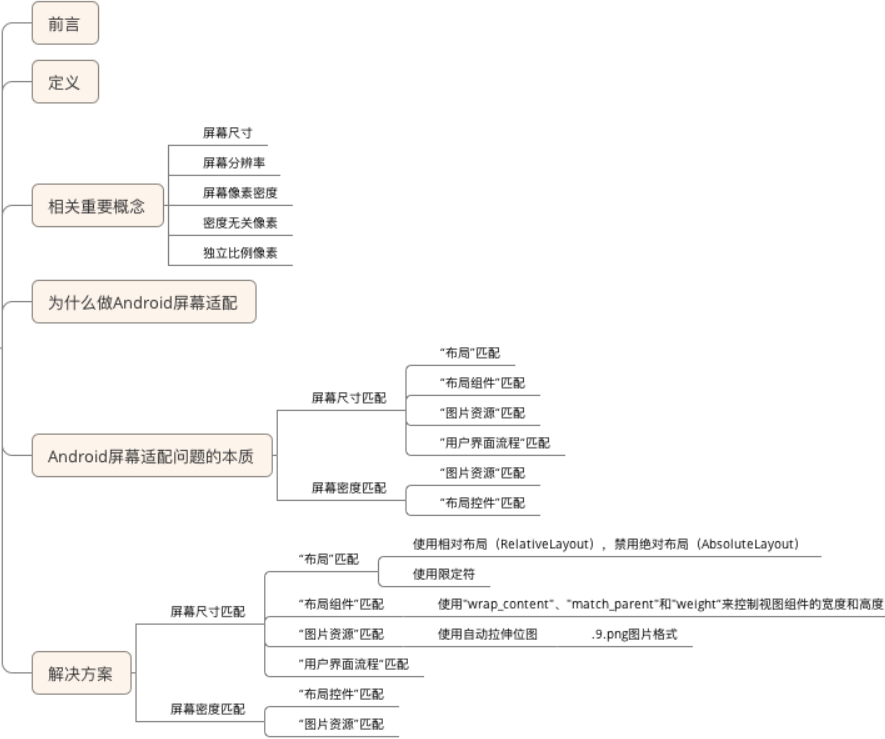
\includegraphics[width=.9\linewidth]{./pic/screenAdapter.png}
\caption{Android屏幕适配解决方案}
\end{figure}

\subsection{定义}
\label{sec-1-3}
\begin{itemize}
\item 使得某一元素在Android不同尺寸、不同分辨率的手机上具备相同的显示效果
\end{itemize}
\subsection{相关重要概念}
\label{sec-1-4}
\subsubsection{屏幕尺寸}
\label{sec-1-4-1}
\begin{itemize}
\item 含义:手机对角线的物理尺寸
\item 单位:英寸(inch),1英寸=2.54cm
\begin{itemize}
\item Android手机常见的尺寸有5寸、5.5寸、6寸等等
\end{itemize}
\end{itemize}
\subsubsection{屏幕分辨率}
\label{sec-1-4-2}
\begin{itemize}
\item 含义:手机在横向、纵向上的像素点数总和
\begin{itemize}
\item 一般描述成屏幕的"宽x高"=AxB
\item 含义:屏幕在横向方向(宽度)上有A个像素点,在纵向方向(高)有B个像素点
\item 例子:1080x1920,即宽度方向上有1080个像素点,在高度方向上有1920个像素点
\end{itemize}
\item 单位:px(pixel),1px=1像素点
\begin{itemize}
\item UI设计师的设计图会以px作为统一的计量单位
\end{itemize}
\item Android手机常见的分辨率:320x480、480x800、720x1280、1080x1920
\end{itemize}
\subsubsection{屏幕像素密度}
\label{sec-1-4-3}
\begin{itemize}
\item 含义:每英寸的像素点数
\item 单位:dpi(dots per ich)
\begin{itemize}
\item 假设设备内每英寸有160个像素,那么该设备的屏幕像素密度=160dpi
\end{itemize}
\item 安卓手机对于每类手机屏幕大小都有一个相应的屏幕像素密度:
\end{itemize}
\begin{center}
\begin{tabular}{lrr}
\hline
密度类型 & 代表的分辨率(px) & 屏幕像素密度(dpi)\\
\hline
低密度(ldpi) & 240x320 & 120\\
中密度(mdpi) & 320x480 & 160\\
高密度(hdpi) & 480x800 & 240\\
超高密度(xhdpi) & 720x1280 & 320\\
超超高密度(xxhdpi) & 1080x1920 & 480\\
\hline
\end{tabular}
\end{center}
\begin{enumerate}
\item 屏幕尺寸、分辨率、像素密度三者关系
\label{sec-1-4-3-1}
\begin{itemize}
\item 一部手机的分辨率是宽x高,屏幕大小是以寸为单位,那么三者的关系是:

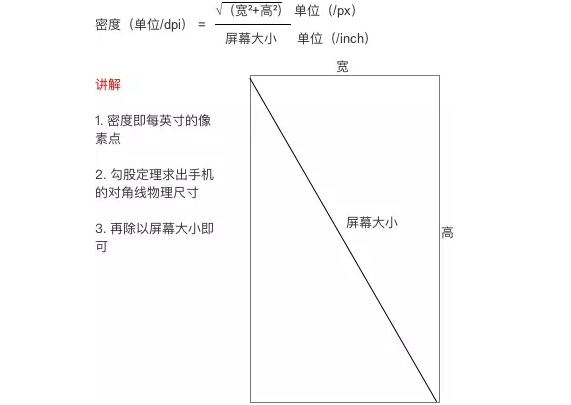
\includegraphics[width=.9\linewidth]{./pic/density2.png}

\item 假设一部手机的分辨率是1080x1920(px),屏幕大小是5寸,问密度是多少?

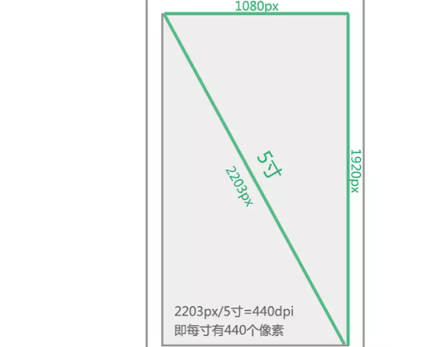
\includegraphics[width=.9\linewidth]{./pic/density3.png}
\end{itemize}
\end{enumerate}

\subsubsection{密度无关像素}
\label{sec-1-4-4}
\begin{itemize}
\item 含义:density-independent pixel,叫dp或dip,与终端上的实际物理像素点无关。
\item 单位:dp,可以保证在不同屏幕像素密度的设备上显示相同的效果
\begin{itemize}
\item Android开发时用dp而不是px单位设置图片大小,是Android特有的单位
\item 场景:假如同样都是画一条长度是屏幕一半的线,如果使用px作为计量单位,那么在480x800分辨率手机上设置应为240px;在320x480的手机上应设置为160px,二者设置就不同了;如果使用dp为单位,在这两种分辨率下,160dp都显示为屏幕一半的长度。
\end{itemize}
\item dp与px的转换
\begin{itemize}
\item 因为ui设计师给你的设计图是以px为单位的,Android开发则是使用dp作为单位的,那么我们需要进行转换:
\end{itemize}
\end{itemize}
\begin{center}
\begin{tabular}{lrrlr}
\hline
密度类型 & 代表的分辨率(px) & 屏幕密度(dpi) & 换算(px/dp) & 比例\\
\hline
低密度(ldpi) & 240x320 & 120 & 1dp=0.75px & 3\\
中密度(mdpi) & 320x480 & 160 & 1dp=1px & 4\\
高密度(hdpi) & 480x800 & 240 & 1dp=1.5px & 6\\
超高密度(xhdpi) & 720x1280 & 320 & 1dp=2px & 8\\
超超高密度(xxhdpi) & 1080x1920 & 480 & 1dp=3px & 12\\
\hline
\end{tabular}
\end{center}
\begin{itemize}
\item 在Android中,规定以160dpi(即屏幕分辨率为320x480)为基准:1dp=1px
\end{itemize}

\subsubsection{独立比例像素}
\label{sec-1-4-5}
\begin{itemize}
\item 含义:scale-independent pixel,叫sp或sip
\item 单位:sp
\begin{itemize}
\item Android开发时用此单位设置文字大小,可根据字体大小首选项进行缩放
\item 推荐使用12sp、14sp、18sp、22sp作为字体设置的大小,不推荐使用奇数和小数,容易造成精度的丢失问题;小于12sp的字体会太小导致用户看不清
\end{itemize}
\end{itemize}

\subsection{为什么要进行Android屏幕适配}
\label{sec-1-5}

由于Android系统的开放性,任何用户、开发者、OEM厂商、运营商都可以对Android进行定制,于是导致:
\begin{itemize}
\item Android系统碎片化:小米定制的MIUI、魅族定制的flyme、华为定制的EMUI等等
\begin{itemize}
\item 当然都是基于Google原生系统定制的
\end{itemize}
\item Android机型屏幕尺寸碎片化:5寸、5.5寸、6寸等等
\item Android屏幕分辨率碎片化:320x480、480x800、720x1280、1080x1920
\begin{itemize}
\item 据友盟指数显示,统计至2015年12月,支持Android的设备共有27796种
\end{itemize}
\item 当Android系统、屏幕尺寸、屏幕密度出现碎片化的时候,就很容易出现同一元素在不同手机上显示不同的问题。
\begin{itemize}
\item 试想一下这么一个场景:
\item 为4.3寸屏幕准备的UI设计图,运行在5.0寸的屏幕上,很可能在右侧和下侧存在大量的空白;而5.0寸的UI设计图运行到4.3寸的设备上,很可能显示不下。
\end{itemize}
\end{itemize}

为了保证用户获得一致的用户体验效果:
\begin{itemize}
\item 使得某一元素在Android不同尺寸、不同分辨率的手机上具备相同的显示效果
\item 于是,我们便需要对Android屏幕进行适配。
\end{itemize}

\subsection{屏幕适配问题的本质}
\label{sec-1-6}
\begin{itemize}
\item 使得"布局"、"布局组件"、"图片资源"、"用户界面流程"匹配不同的屏幕尺寸
\begin{itemize}
\item 使得布局、布局组件自适应屏幕尺寸;
\item 根据屏幕的配置来加载相应的UI布局、用户界面流程
\end{itemize}
\item 使得"图片资源"匹配不同的屏幕密度
\end{itemize}

\subsubsection{屏幕尺寸匹配}
\label{sec-1-6-1}

问题:如何进行屏幕尺寸匹配?

\begin{figure}[htb]
\centering
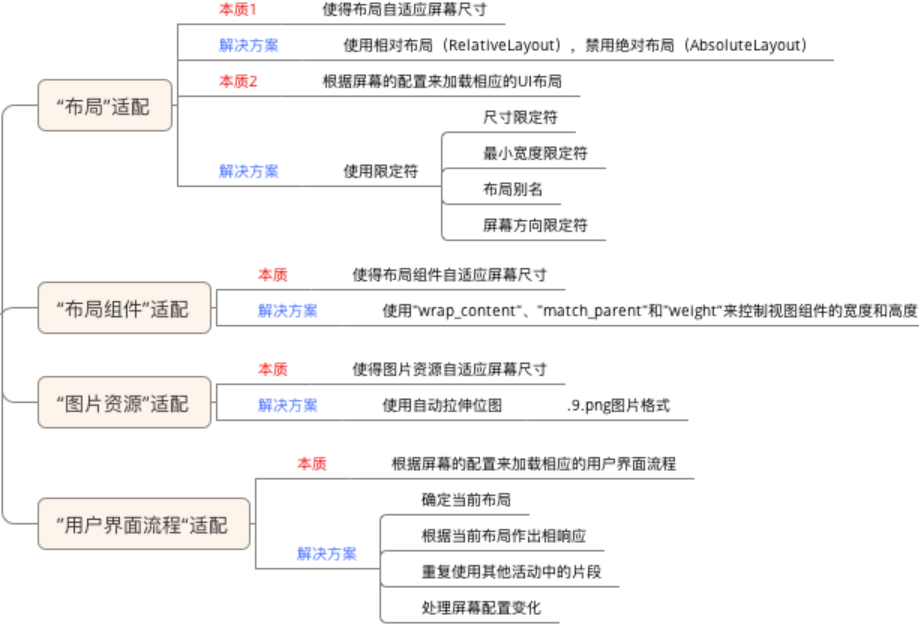
\includegraphics[width=.9\linewidth]{./pic/screenSize.png}
\caption{屏幕尺寸适配解决方案}
\end{figure}

\begin{enumerate}
\item "布局"匹配
\label{sec-1-6-1-1}
\begin{itemize}
\item \textbf{本质1:使得布局元素自适应屏幕尺寸}
\end{itemize}
\begin{enumerate}
\item 使用相对布局(RelativeLayout),禁用绝对布局(AbsoluteLayout)
\label{sec-1-6-1-1-1}

开发中,我们使用的布局一般有:
\begin{itemize}
\item 线性布局(Linearlayout)
\item 相对布局(RelativeLayout)
\item 帧布局(FrameLayout)
\item 绝对布局(AbsoluteLayout)
\begin{itemize}
\item 由于绝对布局(AbsoluteLayout)适配性极差,所以极少使用。
\end{itemize}
\end{itemize}

对于线性布局(Linearlayout)、相对布局(RelativeLayout)和帧布局(FrameLayout)需要根据需求进行选择,但要记住:
\begin{itemize}
\item RelativeLayout
\begin{itemize}
\item 布局的子控件之间使用相对位置的方式排列,因为RelativeLayout讲究的是相对位置,即使屏幕的大小改变,视图之前的相对位置都不会变化,与屏幕大小无关,灵活性很强
\end{itemize}
\item LinearLayout
\begin{itemize}
\item 通过多层嵌套LinearLayout和组合使
\item 用"wrap\_content"和"match\_parent"已经可以构建出足够复杂的布局。但是LinearLayout无法准确地控制子视图之间的位置关系,只能简单的一个挨着一个地排列
\end{itemize}
\end{itemize}

所以,对于屏幕适配来说,使用相对布局(RelativeLayout)将会是更好的解决方案

\begin{itemize}
\item \textbf{本质2:根据屏幕的配置来加载相应的UI布局}
\begin{itemize}
\item 应用场景:需要为不同屏幕尺寸的设备设计不同的布局
\end{itemize}
\end{itemize}
\item 使用限定符
\label{sec-1-6-1-1-2}
\begin{itemize}
\item 作用:通过配置限定符使得程序在运行时根据当前设备的配置(屏幕尺寸)自动加载合适的布局资源
\end{itemize}

限定符类型:
\begin{itemize}
\item 尺寸(size)限定符
\item 最小宽度(Smallest-width)限定符
\item 布局别名
\item 屏幕方向(Orientation)限定符
\end{itemize}

\begin{enumerate}
\item 尺寸(size)限定符
\label{sec-1-6-1-1-2-1}

使用场景:当一款应用显示的内容较多,希望进行以下设置:
\begin{itemize}
\item 在平板电脑和电视的屏幕(>7英寸)上:实施"双面板"模式以同时显示更多内容
\item 在手机较小的屏幕上:使用单面板分别显示内容
\end{itemize}

因此,我们可以使用尺寸限定符(layout-large)通过创建一个文件

\begin{minted}[frame=lines,fontsize=\scriptsize,linenos=false]{xml}
res/layout-large/main.xml
\end{minted}

来完成上述设定:
\begin{itemize}
\item 让系统在屏幕尺寸>7英寸时采用适配平板的双面板布局
\item 反之(默认情况下)采用适配手机的单面板布局
\end{itemize}

文件配置如下:
\begin{itemize}
\item 适配手机的单面板(默认)布局:res/layout/main.xml
\begin{minted}[frame=lines,fontsize=\scriptsize,linenos=false]{xml}
<LinearLayout xmlns:android="http://schemas.android.com/apk/res/android"
      android:orientation="vertical"
      android:layout_width="match_parent"
      android:layout_height="match_parent">
      <fragment android:id="@+id/headlines"
          android:layout_height="fill_parent"
          android:name="com.example.android.newsreader.HeadlinesFragment"
          android:layout_width="match_parent"
      />
</LinearLayout>
\end{minted}
\item 适配尺寸>7寸平板的双面板布局::res/layout-large/main.xml
\begin{minted}[frame=lines,fontsize=\scriptsize,linenos=false]{xml}
<LinearLayout xmlns:android="http://schemas.android.com/apk/res/android"
    android:layout_width="fill_parent"
    android:layout_height="fill_parent"
    android:orientation="horizontal">
    <fragment android:id="@+id/headlines"
        android:layout_height="fill_parent"
        android:name="com.example.android.newsreader.HeadlinesFragment"
        android:layout_width="400dp"
        android:layout_marginRight="10dp"
    />
    <fragment android:id="@+id/article"
        android:layout_height="fill_parent"
        android:name="com.example.android.newsreader.ArticleFragment"
        android:layout_width="fill_parent"
    />
</LinearLayout>
\end{minted}
\end{itemize}

请注意:
\begin{itemize}
\item 两个布局名称均为main.xml,只有布局的目录名不同:第一个布局的目录名为:layout,第二个布局的目录名为:layout-large,包含了尺寸限定符(large)
\item 被定义为大屏的设备(7寸以上的平板)会自动加载包含了large限定符目录的布局,而小屏设备会加载另一个默认的布局
\end{itemize}

\textbf{但要注意的是,这种方式只适合Android 3.2版本之前。}

\item 最小宽度(Smallest-width)限定符
\label{sec-1-6-1-1-2-2}
\begin{itemize}
\item 背景:上述提到的限定符"large"具体是指多大呢?似乎没有一个定量的指标,这便意味着可能没办法准确地根据当前设备的配置(屏幕尺寸)自动加载合适的布局资源
\item 例子:比如说large同时包含着5寸和7寸,这意味着使用"large"限定符的话我没办法实现为5寸和7寸的平板电脑分别加载不同的布局
\end{itemize}

于是,在Android 3.2及之后版本,引入了最小宽度(Smallest-width)限定符
\begin{itemize}
\item 定义:通过指定某个最小宽度(以 dp 为单位)来精确定位屏幕从而加载不同的UI资源
\item 使用场景:
\begin{itemize}
\item 你需要为标准 7 英寸平板电脑匹配双面板布局(其最小宽度为 600 dp),在手机(较小的屏幕上)匹配单面板布局
\end{itemize}
\item 解决方案:
\begin{itemize}
\item 您可以使用上文中所述的单面板和双面板这两种布局,但您应使用 sw600dp 指明双面板布局仅适用于最小宽度为 600 dp 的屏幕,而不是使用 large 尺寸限定符。
\begin{itemize}
\item sw xxxdp,即small width的缩写,其不区分方向,即无论是宽度还是高度,只要大于 xxxdp,就采用次此布局
\end{itemize}
\end{itemize}
\item 例子:
\begin{itemize}
\item 使用了layout-sw 600dp的最小宽度限定符,即无论是宽度还是高度,只要大于600dp,就采用layout-sw 600dp目录下的布局
\end{itemize}
\end{itemize}

代码展示:
\begin{itemize}
\item 适配手机的单面板(默认)布局:res/layout/main.xml
\begin{minted}[frame=lines,fontsize=\scriptsize,linenos=false]{xml}
<LinearLayout xmlns:android="http://schemas.android.com/apk/res/android"
    android:orientation="vertical"
    android:layout_width="match_parent"
    android:layout_height="match_parent">
    <fragment android:id="@+id/headlines"
        android:layout_height="fill_parent"
        android:name="com.example.android.newsreader.HeadlinesFragment"
        android:layout_width="match_parent" />
</LinearLayout>
\end{minted}
\item 适配尺寸>7寸平板的双面板布局:res/layout-sw600dp/main.xml
\begin{minted}[frame=lines,fontsize=\scriptsize,linenos=false]{xml}
<LinearLayout xmlns:android="http://schemas.android.com/apk/res/android"
    android:layout_width="fill_parent"
    android:layout_height="fill_parent"
    android:orientation="horizontal">
    <fragment android:id="@+id/headlines"
          android:layout_height="fill_parent"
          android:name="com.example.android.newsreader.HeadlinesFragment"
          android:layout_width="400dp"
          android:layout_marginRight="10dp"/>
    <fragment android:id="@+id/article"
          android:layout_height="fill_parent"
          android:name="com.example.android.newsreader.ArticleFragment"
          android:layout_width="fill_parent" />
</LinearLayout>
\end{minted}
\item 对于最小宽度≥ 600 dp 的设备
\begin{itemize}
\item 系统会自动加载 layout-sw600dp/main.xml(双面板)布局,否则系统就会选择 layout/main.xml(单面板)布局
\item (这个选择过程是Android系统自动选择的)
\end{itemize}
\end{itemize}
\item 使用布局别名
\label{sec-1-6-1-1-2-3}

\textbf{设想这么一个场景}

当你需要同时为Android 3.2版本前和Android 3.2版本后的手机进行屏幕尺寸适配的时候,由于尺寸限定符仅用于Android 3.2版本前,最小宽度限定符仅用于Android 3.2版本后,所以这会带来一个问题,为了很好地进行屏幕尺寸的适配,你需要同时维护layout-sw600dp和layout-large的两套main.xml平板布局,如下:
\begin{itemize}
\item 适配手机的单面板(默认)布局:res/layout/main.xml
\item 适配尺寸>7寸平板的双面板布局(Android 3.2前):res/layout-large/main.xml
\item 适配尺寸>7寸平板的双面板布局(Android 3.2后)res/layout-sw600dp/main.xml
\end{itemize}

最后的两个文件的xml内容是完全相同的,这会带来:文件名的重复从而带来一些列后期维护的问题

\textbf{于是为了要解决这种重复问题,我们引入了--布局别名} 

还是上面的例子,你可以定义以下布局:
\begin{itemize}
\item 适配手机的单面板(默认)布局:res/layout/main.xml
\item 适配尺寸>7寸平板的双面板布局:res/layout/main\_twopanes.xml
\end{itemize}

然后加入以下两个文件,以便进行Android 3.2前和Android 3.2后的版本双面板布局适配:
\begin{itemize}
\item res/values-large/layout.xml(Android 3.2之前的双面板布局)
\begin{minted}[frame=lines,fontsize=\scriptsize,linenos=false]{xml}
<resources>
    <item name="main" type="layout">@layout/main_twopanes</item>
</resources>
\end{minted}
\item res/values-sw600dp/layout.xml(Android 3.2及之后的双面板布局)
\begin{minted}[frame=lines,fontsize=\scriptsize,linenos=false]{xml}
<resources>
    <item name="main" type="layout">@layout/main_twopanes</item>
</resources>
\end{minted}
\end{itemize}

注:
\begin{itemize}
\item 最后两个文件有着相同的内容,但是它们并没有真正去定义布局,它们仅仅只是将main设置成了@layout/main\_twopanes的别名
\item 由于这些文件包含 large 和 sw600dp 选择器,因此,系统会将此文件匹配到不同版本的>7寸平板上:
\begin{itemize}
\item a. 版本低于 3.2 的平板会匹配 large的文件
\item b. 版本高于 3.2 的平板会匹配 sw600dp的文件
\end{itemize}
\end{itemize}

这样两个layout.xml都只是引用了@layout/main\_twopanes,就避免了重复定义布局文件的情况

\item 屏幕方向(Orientation)限定符
\label{sec-1-6-1-1-2-4}
\begin{itemize}
\item 使用场景:根据屏幕方向进行布局的调整
\item 取以下为例子:
\begin{itemize}
\item 小屏幕, 竖屏: 单面板
\item 小屏幕, 横屏: 单面板
\item 7 英寸平板电脑,纵向:单面板,带操作栏
\item 7 英寸平板电脑,横向:双面板,宽,带操作栏
\item 10 英寸平板电脑,纵向:双面板,窄,带操作栏
\item 10 英寸平板电脑,横向:双面板,宽,带操作栏
\item 电视,横向:双面板,宽,带操作栏
\end{itemize}
\item 方法是
\begin{itemize}
\item 先定义类别:单/双面板、是否带操作栏、宽/窄
\begin{itemize}
\item 定义在 res/layout/ 目录下的某个 XML 文件中
\end{itemize}
\item 再进行相应的匹配:屏幕尺寸(小屏、7寸、10寸)、方向(横、纵)
\begin{itemize}
\item 使用布局别名进行匹配
\end{itemize}
\end{itemize}
\item \textbf{在 res/layout/ 目录下的某个 XML 文件中定义所需要的布局类别}
\begin{itemize}
\item (单/双面板、是否带操作栏、宽/窄)
\item res/layout/onepane.xml:(单面板)
\end{itemize}
\begin{minted}[frame=lines,fontsize=\scriptsize,linenos=false]{xml}
<LinearLayout xmlns:android="http://schemas.android.com/apk/res/android"  
    android:orientation="vertical"  
    android:layout_width="match_parent"  
    android:layout_height="match_parent">  
    <fragment android:id="@+id/headlines"  
          android:layout_height="fill_parent"  
          android:name="com.example.android.newsreader.HeadlinesFragment"  
          android:layout_width="match_parent" />  
</LinearLayout>
\end{minted}
\begin{itemize}
\item res/layout/onepane\_with\_bar.xml:(单面板带操作栏)
\end{itemize}
\begin{minted}[frame=lines,fontsize=\scriptsize,linenos=false]{xml}
<LinearLayout xmlns:android="http://schemas.android.com/apk/res/android"  
    android:orientation="vertical"  
    android:layout_width="match_parent"  
    android:layout_height="match_parent">  
    <LinearLayout android:layout_width="match_parent"   
          android:id="@+id/linearLayout1"    
          android:gravity="center"  
          android:layout_height="50dp">  
        <ImageView android:id="@+id/imageView1"   
               android:layout_height="wrap_content"  
               android:layout_width="wrap_content"  
               android:src="@drawable/logo"  
               android:paddingRight="30dp"  
               android:layout_gravity="left"  
               android:layout_weight="0" />  
        <View android:layout_height="wrap_content"   
              android:id="@+id/view1"  
              android:layout_width="wrap_content"  
              android:layout_weight="1" />  
        <Button android:id="@+id/categorybutton"  
            android:background="@drawable/button_bg"  
            android:layout_height="match_parent"  
            android:layout_weight="0"  
            android:layout_width="120dp"  
            style="@style/CategoryButtonStyle"/>  
    </LinearLayout>  
    <fragment android:id="@+id/headlines"   
          android:layout_height="fill_parent"  
          android:name="com.example.android.newsreader.HeadlinesFragment"  
          android:layout_width="match_parent" 
    />  
</LinearLayout>
\end{minted}
\begin{itemize}
\item res/layout/twopanes.xml:(双面板,宽布局)
\end{itemize}
\begin{minted}[frame=lines,fontsize=\scriptsize,linenos=false]{xml}
<LinearLayout xmlns:android="http://schemas.android.com/apk/res/android"
    android:layout_width="fill_parent"
    android:layout_height="fill_parent"
    android:orientation="horizontal">
    <fragment android:id="@+id/headlines"
          android:layout_height="fill_parent"
          android:name="com.example.android.newsreader.HeadlinesFragment"
          android:layout_width="400dp"
          android:layout_marginRight="10dp"/>
    <fragment android:id="@+id/article"
          android:layout_height="fill_parent"
          android:name="com.example.android.newsreader.ArticleFragment"
          android:layout_width="fill_parent" />
</LinearLayout>
\end{minted}
\begin{itemize}
\item res/layout/twopanes\_narrow.xml:(双面板,窄布局)
\end{itemize}
\begin{minted}[frame=lines,fontsize=\scriptsize,linenos=false]{xml}
<LinearLayout xmlns:android="http://schemas.android.com/apk/res/android"
    android:layout_width="fill_parent"
    android:layout_height="fill_parent"
    android:orientation="horizontal">
    <fragment android:id="@+id/headlines"
          android:layout_height="fill_parent"
          android:name="com.example.android.newsreader.HeadlinesFragment"
          android:layout_width="200dp"
          android:layout_marginRight="10dp"/>
    <fragment android:id="@+id/article"
          android:layout_height="fill_parent"
          android:name="com.example.android.newsreader.ArticleFragment"
          android:layout_width="fill_parent" />
</LinearLayout>
\end{minted}
\item \textbf{使用布局别名进行相应的匹配}
\begin{itemize}
\item (屏幕尺寸(小屏、7寸、10寸)、方向(横、纵))
\item res/values/layouts.xml:(默认布局)
\end{itemize}
\begin{minted}[frame=lines,fontsize=\scriptsize,linenos=false]{xml}
<resources>  
    <item name="main_layout" type="layout">@layout/onepane_with_bar</item>  
    <bool name="has_two_panes">false</bool>  
</resources>
\end{minted}
\begin{itemize}
\item 可为resources设置bool,通过获取其值来动态判断目前已处在哪个适配布局
\item res/values-sw600dp-land/layouts.xml
\begin{itemize}
\item (大屏、横向、双面板、宽-Andorid 3.2版本后)
\end{itemize}
\end{itemize}
\begin{minted}[frame=lines,fontsize=\scriptsize,linenos=false]{xml}
<resources>
    <item name="main_layout" type="layout">@layout/twopanes</item>
    <bool name="has_two_panes">true</bool>
</resources>
\end{minted}
\begin{itemize}
\item res/values-sw600dp-port/layouts.xml
\begin{itemize}
\item (大屏、纵向、单面板带操作栏-Andorid 3.2版本后)
\end{itemize}
\end{itemize}
\begin{minted}[frame=lines,fontsize=\scriptsize,linenos=false]{xml}
<resources>
    <item name="main_layout" type="layout">@layout/onepane</item>
    <bool name="has_two_panes">false</bool>
</resources>
\end{minted}
\begin{itemize}
\item res/values-large-land/layouts.xml
\begin{itemize}
\item (大屏、横向、双面板、宽-Andorid 3.2版本前)
\end{itemize}
\end{itemize}
\begin{minted}[frame=lines,fontsize=\scriptsize,linenos=false]{xml}
<resources>
    <item name="main_layout" type="layout">@layout/twopanes</item>
    <bool name="has_two_panes">true</bool>
</resources>
\end{minted}
\begin{itemize}
\item res/values-large-port/layouts.xml
\begin{itemize}
\item (大屏、纵向、单面板带操作栏-Andorid 3.2版本前)
\end{itemize}
\end{itemize}
\begin{minted}[frame=lines,fontsize=\scriptsize,linenos=false]{xml}
<resources>
    <item name="main_layout" type="layout">@layout/onepane</item>
    <bool name="has_two_panes">false</bool>
</resources>
\end{minted}
\begin{itemize}
\item 这里没有完全把全部尺寸匹配类型的代码贴出来,大家可以自己去尝试把其补充完整
\end{itemize}
\end{itemize}
\end{enumerate}
\end{enumerate}

\item "布局组件"匹配
\label{sec-1-6-1-2}

\textbf{本质:使得布局组件自适应屏幕尺寸}
\begin{itemize}
\item 做法: 使用"wrap\_content"、"match\_parent"和"weight"来控制视图组件的宽度和高度
\begin{itemize}
\item "wrap\_content"
\begin{itemize}
\item 相应视图的宽和高就会被设定成所需的最小尺寸以适应视图中的内容
\end{itemize}
\item "match\_parent"(在Android API 8之前叫作"fill\_parent")
\begin{itemize}
\item 视图的宽和高延伸至充满整个父布局
\end{itemize}
\item "weight"
\begin{itemize}
\item 1.定义:是线性布局(Linelayout)的一个独特比例分配属性
\item 2.作用:使用此属性设置权重,然后按照比例对界面进行空间的分配,公式计算是:控件宽度=控件设置宽度+剩余空间所占百分比宽幅
\item 具体可以参考这篇文章,讲解得非常详细 \url{http://mobile.51cto.com/abased-375428.htm}
\end{itemize}
\end{itemize}
\end{itemize}

通过使用"wrap\_content"、"match\_parent"和"weight"来替代硬编码的方式定义视图大小\&位置,你的视图要么仅仅使用了需要的那边一点空间,要么就会充满所有可用的空间,即按需占据空间大小,能让你的布局元素充分适应你的屏幕尺寸

\item "图片资源"匹配
\label{sec-1-6-1-3}

\textbf{本质:使得图片资源在不同屏幕密度上显示相同的像素效果}
\begin{itemize}
\item 做法: \textbf{使用自动拉伸位图:Nine-Patch的图片类型}
\begin{itemize}
\item 假设需要匹配不同屏幕大小,你的图片资源也必须自动适应各种屏幕尺寸
\begin{itemize}
\item 使用场景:一个按钮的背景图片必须能够随着按钮大小的改变而改变。
\item 使用普通的图片将无法实现上述功能,因为运行时会均匀地拉伸或压缩你的图片
\end{itemize}
\end{itemize}
\item 解决方案:使用自动拉伸位图(nine-patch图片),后缀名是.9.png,它是一种被特殊处理过的PNG图片,设计时可以指定图片的拉伸区域和非拉伸区域;使用时,系统就会根据控件的大小自动地拉伸你想要拉伸的部分
\begin{itemize}
\item 1.必须要使用.9.png后缀名,因为系统就是根据这个来区别nine-patch图片和普通的PNG图片的;
\item 2.当你需要在一个控件中使用nine-patch图片时,如
\end{itemize}
\begin{minted}[frame=lines,fontsize=\scriptsize,linenos=false]{xml}
android:background="@drawable/button"
\end{minted}
\end{itemize}

系统就会根据控件的大小自动地拉伸你想要拉伸的部分

\item "用户界面流程"匹配
\label{sec-1-6-1-4}
\begin{itemize}
\item 使用场景:我们会根据设备特点显示恰当的布局,但是这样做,会使得用户界面流程可能会有所不同。
\item 例如,如果应用处于双面板模式下,点击左侧面板上的项即可直接在右侧面板上显示相关内容;而如果该应用处于单面板模式下,点击相关的内容应该跳转到另外一个Activity进行后续的处理。
\end{itemize}

\textbf{本质:根据屏幕的配置来加载相应的用户界面流程}
\begin{itemize}
\item 做法:进行用户界面流程的自适应配置:
\begin{itemize}
\item 确定当前布局
\item 根据当前布局做出响应
\item 重复使用其他活动中的片段
\item 处理屏幕配置变化
\end{itemize}
\item 步骤1:确定当前布局
\begin{itemize}
\item 由于每种布局的实施都会稍有不同,因此我们需要先确定当前向用户显示的布局。例如,我们可以先了解用户所处的是"单面板"模式还是"双面板"模式。要做到这一点,可以通过查询指定视图是否存在以及是否已显示出来。
\end{itemize}
\begin{minted}[frame=lines,fontsize=\scriptsize,linenos=false]{java}
public class NewsReaderActivity extends FragmentActivity {
    boolean mIsDualPane;
    @Override
    public void onCreate(Bundle savedInstanceState) {
        super.onCreate(savedInstanceState);
        setContentView(R.layout.main_layout);
        View articleView = findViewById(R.id.article);
        mIsDualPane = articleView != null &&
                        articleView.getVisibility() == View.VISIBLE;
    }
}
\end{minted}
\begin{itemize}
\item 这段代码用于查询"报道"面板是否可用,与针对具体布局的硬编码查询相比,这段代码的灵活性要大得多。
\end{itemize}
\item 步骤2:根据当前布局做出响应
\begin{itemize}
\item 有些操作可能会因当前的具体布局而产生不同的结果。
\item 例如,在新闻阅读器示例中,如果用户界面处于双面板模式下,那么点击标题列表中的标题就会在右侧面板中打开相应报道;但如果用户界面处于单面板模式下,那么上述操作就会启动一个独立活动:
\end{itemize}
\begin{minted}[frame=lines,fontsize=\scriptsize,linenos=false]{java}
@Override
public void onHeadlineSelected(int index) {
    mArtIndex = index;
    if (mIsDualPane) {
        /* display article on the right pane */
        mArticleFragment.displayArticle(mCurrentCat.getArticle(index));
    } else {
        /* start a separate activity */
        Intent intent = new Intent(this, ArticleActivity.class);
        intent.putExtra("catIndex", mCatIndex);
        intent.putExtra("artIndex", index);
        startActivity(intent);
    }
}
\end{minted}
\item 步骤3:重复使用其他活动中的片段
\begin{itemize}
\item 多屏幕设计中的重复模式是指,对于某些屏幕配置,已实施界面的一部分会用作面板;但对于其他配置,这部分就会以独立活动的形式存在。
\begin{itemize}
\item 例如,在新闻阅读器示例中,对于较大的屏幕,新闻报道文本会显示在右侧面板中;但对于较小的屏幕,这些文本就会以独立活动的形式存在。
\end{itemize}
\item 在类似情况下,通常可以在多个活动中重复使用相同的 Fragment 子类以避免代码重复。例如,在双面板布局中使用了 ArticleFragment:
\end{itemize}
\begin{minted}[frame=lines,fontsize=\scriptsize,linenos=false]{xml}
<LinearLayout xmlns:android="http://schemas.android.com/apk/res/android"
    android:layout_width="fill_parent"
    android:layout_height="fill_parent"
    android:orientation="horizontal">
    <fragment android:id="@+id/headlines"
          android:layout_height="fill_parent"
          android:name="com.example.android.newsreader.HeadlinesFragment"
          android:layout_width="400dp"
          android:layout_marginRight="10dp"/>
    <fragment android:id="@+id/article"
          android:layout_height="fill_parent"
          android:name="com.example.android.newsreader.ArticleFragment"
          android:layout_width="fill_parent" />
</LinearLayout>
\end{minted}
\begin{itemize}
\item 然后又在小屏幕的Activity布局中重复使用了它 :
\end{itemize}
\begin{minted}[frame=lines,fontsize=\scriptsize,linenos=false]{java}
ArticleFragment frag = new ArticleFragment();
getSupportFragmentManager().beginTransaction().
    add(android.R.id.content, frag).commit();
\end{minted}
\item 步骤4:处理屏幕配置变化
\begin{itemize}
\item 如果我们使用独立Activity实施界面的独立部分,那么请注意,我们可能需要对特定配置变化(例如屏幕方向的变化)做出响应,以便保持界面的一致性。
\begin{itemize}
\item 例如,在运行 Android 3.0 或更高版本的标准 7 英寸平板电脑上,如果新闻阅读器示例应用运行在纵向模式下,就会在使用独立活动显示新闻报道;但如果该应用运行在横向模式下,就会使用双面板布局。
\end{itemize}
\item 也就是说,如果用户处于纵向模式下且屏幕上显示的是用于阅读报道的活动,那么就需要在检测到屏幕方向变化(变成横向模式)后执行相应操作,即停止上述活动并返回主活动,以便在双面板布局中显示相关内容:
\end{itemize}
\begin{minted}[frame=lines,fontsize=\scriptsize,linenos=false]{java}
public class ArticleActivity extends FragmentActivity {
    int mCatIndex, mArtIndex;
    @Override
    protected void onCreate(Bundle savedInstanceState) {
        super.onCreate(savedInstanceState);
        mCatIndex = getIntent().getExtras().getInt("catIndex", 0);
        mArtIndex = getIntent().getExtras().getInt("artIndex", 0);
        // If should be in two-pane mode, finish to return to main activity
        if (getResources().getBoolean(R.bool.has_two_panes)) {
            finish();
            return;
        }
        ...
}
\end{minted}
\end{itemize}

通过上面一系列步骤,我们就完全可以建立一个可以根据用户界面配置进行自适应的应用程序App了。
\end{enumerate}

\subsubsection{屏幕密度匹配}
\label{sec-1-6-2}

问题:如何进行屏幕密度匹配?

\begin{figure}[htb]
\centering
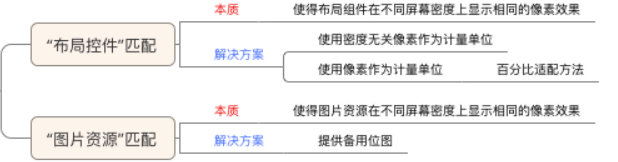
\includegraphics[width=.9\linewidth]{./pic/density.png}
\caption{屏幕密度匹配解决方案}
\end{figure}

\begin{enumerate}
\item "布局控件"匹配
\label{sec-1-6-2-1}

\textbf{本质:使得布局组件在不同屏幕密度上显示相同的像素效果}
\begin{enumerate}
\item 使用密度无关像素作为计量单位
\label{sec-1-6-2-1-1}
\begin{itemize}
\item 由于各种屏幕的像素密度都有所不同,因此相同数量的像素在不同设备上的实际大小也有所差异,这样使用像素(px)定义布局尺寸就会产生问题。
\item 因此,请务必使用密度无关像素 dp 或**独立比例像素 sp **单位指定尺寸。
\end{itemize}

\textbf{密度无关像素}
\begin{itemize}
\item 含义:density-independent pixel,叫dp或dip,与终端上的实际物理像素点无关。
\item 单位:dp,可以保证在不同屏幕像素密度的设备上显示相同的效果
\begin{itemize}
\item Android开发时用dp而不是px单位设置图片大小,是Android特有的单位
\item 场景:假如同样都是画一条长度是屏幕一半的线,如果使用px作为计量单位,那么在480x800分辨率手机上设置应为240px;在320x480的手机上应设置为160px,二者设置就不同了;如果使用dp为单位,在这两种分辨率下,160dp都显示为屏幕一半的长度。
\end{itemize}
\item dp与px的转换
\begin{itemize}
\item 因为ui给你的设计图是以px为单位的,Android开发则是使用dp作为单位的,那么该如何转换呢?
\end{itemize}
\end{itemize}
\begin{center}
\begin{tabular}{lrrlr}
\hline
密度类型 & 代表的分辨率(px) & 屏幕密度(dpi) & 换算(px/dp) & 比例\\
\hline
低密度(ldpi) & 240x320 & 120 & 1dp=0.75px & 3\\
中密度(mdpi) & 320x480 & 160 & 1dp=1px & 4\\
高密度(hdpi) & 480x800 & 240 & 1dp=1.5px & 6\\
超高密度(xhdpi) & 720x1280 & 320 & 1dp=2px & 8\\
超超高密度(xxhdpi) & 1080x1920 & 480 & 1dp=3px & 12\\
\hline
\end{tabular}
\end{center}

在Android中,规定以160dpi(即屏幕分辨率为320x480)为基准:1dp=1px

\textbf{独立比例像素}
\begin{itemize}
\item 含义:scale-independent pixel,叫sp或sip
\item 单位:sp
\begin{itemize}
\item Android开发时用此单位设置文字大小,可根据用户的偏好文字大小/字体大小首选项进行缩放
\item 推荐使用12sp、14sp、18sp、22sp作为字体设置的大小,不推荐使用奇数和小数,容易造成精度的丢失问题;小于12sp的字体会太小导致用户看不清
\end{itemize}
\end{itemize}

所以,为了能够进行不同屏幕像素密度的匹配,我们推荐:
\begin{itemize}
\item 使用dp来代替px作为控件长度的统一度量单位
\item 使用sp作为文字的统一度量单位
\end{itemize}

可是,请看以下一种场景:
\begin{itemize}
\item Nexus5的总宽度为360dp,我们现在在水平方向上放置两个按钮,一个是150dp左对齐,另外一个是200dp右对齐,那么中间留有10dp间隔;但假如同样地设置在Nexus S(屏幕宽度是320dp),会发现,两个按钮会重叠,因为320dp<200+150dp
\end{itemize}

从上面可以看出,由于Android屏幕设备的多样性,如果使用dp来作为度量单位,并不是所有的屏幕的宽度都具备相同的dp长度
\begin{itemize}
\item 再次明确, \textbf{屏幕宽度和像素密度没有任何关联关系}
\end{itemize}

所以说,dp解决了同一数值在不同分辨率中展示相同尺寸大小的问题(即屏幕像素密度匹配问题),但却没有解决设备尺寸大小匹配的问题。(即屏幕尺寸匹配问题)
\begin{itemize}
\item 当然,我们一开始讨论的就是屏幕尺寸匹配问题,使用match\_parent、wrap\_content和weight,尽可能少用dp来指定控件的具体长宽,大部分的情况我们都是可以做到适配的。
\end{itemize}

\textbf{那么该如何解决控件的屏幕尺寸和屏幕密度的适配问题呢?}

从上面可以看出:
\begin{itemize}
\item 因为屏幕密度(分辨率)不一样,所以不能用固定的px
\item 因为屏幕宽度不一样,所以要小心的用dp
\end{itemize}

因为本质上是希望使得布局组件在不同屏幕密度上显示相同的像素效果,那么,之前是绕了个弯使用dp解决这个问题,那么到底能不能直接用px解决呢?
\begin{itemize}
\item 即根据不同屏幕密度,控件选择对应的像素值大小
\end{itemize}

\item 百分比适配方法
\label{sec-1-6-2-1-2}
\begin{itemize}
\item 以某一分辨率为基准,生成所有分辨率对应像素数列表
\item 将生成像素数列表存放在res目录下对应的values文件下
\item 根据UI设计师给出设计图上的尺寸,找到对应像素数的单位,然后设置给控件即可
\end{itemize}

\begin{enumerate}
\item 步骤1:以某一分辨率为基准,生成所有分辨率对应像素数列表
\label{sec-1-6-2-1-2-1}

现在我们以320x480的分辨率为基准:
\begin{itemize}
\item 将屏幕的宽度分为320份,取值为x1\textasciitilde{}x320
\item 将屏幕的高度分为480份,取值为y1\textasciitilde{}y480
\end{itemize}

然后生成该分辨率对应像素数的列表,如下图:
\begin{itemize}
\item lay\_x.xml(宽)
\begin{minted}[frame=lines,fontsize=\scriptsize,linenos=false]{xml}
<?xml version="1.0" encoding="utf-8"?>
<resources><dimen name="x1">1.0px</dimen>
    <dimen name="x2">2.0px</dimen>
    <dimen name="x3">3.0px</dimen>
    <dimen name="x4">4.0px</dimen>
    <dimen name="x5">5.0px</dimen>
    <dimen name="x6">6.0px</dimen>
    <dimen name="x7">7.0px</dimen>
    <dimen name="x8">8.0px</dimen>
    <dimen name="x9">9.0px</dimen>
    <dimen name="x10">10.0px</dimen>
    ...
    <dimen name="x300">300.0px</dimen>
    <dimen name="x301">301.0px</dimen>
    <dimen name="x302">302.0px</dimen>
    <dimen name="x303">303.0px</dimen>
    <dimen name="x304">304.0px</dimen>
    <dimen name="x305">305.0px</dimen>
    <dimen name="x306">306.0px</dimen>
    <dimen name="x307">307.0px</dimen>
    <dimen name="x308">308.0px</dimen>
    <dimen name="x309">309.0px</dimen>
    <dimen name="x310">310.0px</dimen>
    <dimen name="x311">311.0px</dimen>
    <dimen name="x312">312.0px</dimen>
    <dimen name="x313">313.0px</dimen>
    <dimen name="x314">314.0px</dimen>
    <dimen name="x315">315.0px</dimen>
    <dimen name="x316">316.0px</dimen>
    <dimen name="x317">317.0px</dimen>
    <dimen name="x318">318.0px</dimen>
    <dimen name="x319">319.0px</dimen>
    <dimen name="x320">320px</dimen>
</resources>
\end{minted}
\item lay\_y.xml(高)
\begin{minted}[frame=lines,fontsize=\scriptsize,linenos=false]{xml}
<?xml version="1.0" encoding="utf-8"?>
<resources><dimen name="y1">1.0px</dimen>
    <dimen name="y2">2.0px</dimen>
    <dimen name="y3">3.0px</dimen>
    <dimen name="y4">4.0px</dimen>
    ...
    <dimen name="y480">480px</dimen>
</resources>
\end{minted}
\end{itemize}

找到基准后,是时候把其他分辨率补全了,现今以写1080x1920的分辨率为例:
\begin{itemize}
\item 因为基准是320x480,所以1080/320=3.375px,1920/480=4px,所以相应文件应该是
\begin{itemize}
\item lay\_x.xml
\end{itemize}
\begin{minted}[frame=lines,fontsize=\scriptsize,linenos=false]{xml}
<?xml version="1.0" encoding="utf-8"?>
<resources><dimen name="x1">3.375px</dimen>
    <dimen name="x2">6.65px</dimen>
    <dimen name="x3">10.125px</dimen>
    ...
    <dimen name="x320">1080px</dimen>
</resources>
\end{minted}
\begin{itemize}
\item lay\_y.xml
\end{itemize}
\begin{minted}[frame=lines,fontsize=\scriptsize,linenos=false]{xml}
<?xml version="1.0" encoding="utf-8"?>
<resources><dimen name="y1">4px</dimen>
    <dimen name="y2">8px</dimen>
    <dimen name="y3">12px</dimen>
    <dimen name="y4">16px</dimen>
    ...
    <dimen name="y480">1920px</dimen>
</resources>
\end{minted}
\end{itemize}

用上面的方法把你需要适配的分辨率的像素列表补全吧\textasciitilde{}

作为程序猿的我们当然不会做手写的这些蠢事!!!多谢 @鸿洋大神 提供了自动生成工具(内置了常用的分辨率),大家可以直接点击这里下载

注:工具默认基准为400*320,当然对于特殊需求,通过命令行指定即可:

\begin{minted}[frame=lines,fontsize=\scriptsize,linenos=false]{xml}
java -jar 文件名.jar 基准宽 基准高 额外支持尺寸1的宽,额外支持尺寸1的高_额外支持尺寸2的宽,额外支持尺寸2的高:
\end{minted}

例如:需要设置的基准是800x1280,额外支持尺寸:735x1152 ;3200x4500;

\begin{minted}[frame=lines,fontsize=\scriptsize,linenos=false]{xml}
java -jar 文件名.jar 800 1280 735,1152_3200,4500
\end{minted}

\item 步骤2:把生成的各像素数列表放到对应的资源文件
\label{sec-1-6-2-1-2-2}

将生成像素数列表(lay\_x.xml和lay\_y.xml)存放在res目录下对应的values文件(注意宽、高要对应),如下图:

\begin{figure}[htb]
\centering
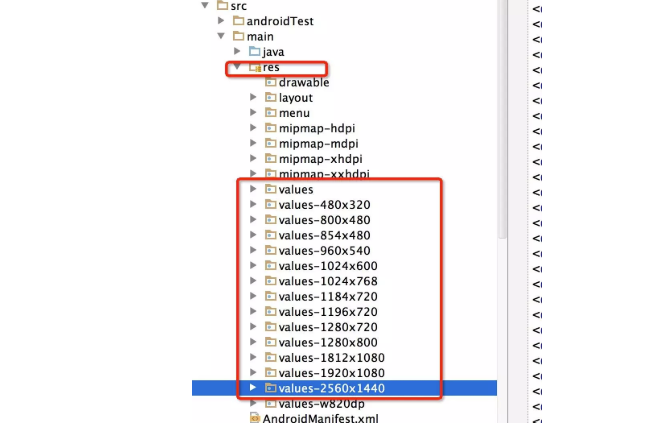
\includegraphics[width=.9\linewidth]{./pic/res.png}
\caption{res目录下对应的values文件}
\end{figure}

注:
\begin{itemize}
\item 分辨率为480x320的资源文件应放在res/values-480x320文件夹中;同理分辨率为1920x1080的资源文件应放在res/values-1920x1080文件夹中。(其中values-480x320是分辨率限定符)
\item 必须在默认values里面也创建对应默认lay\_x.xml和lay\_y.xml文件,如下图
\begin{itemize}
\item lay\_x.xml
\end{itemize}
\begin{minted}[frame=lines,fontsize=\scriptsize,linenos=false]{xml}
<?xml version="1.0" encoding="utf-8">
<resources>
    <dimen name="x1">1.0dp</dimen>
    <dimen name="x2">2.0dp</dimen>
    ...
</resources>
\end{minted}
\item 因为对于没有生成对应分辨率文件的手机,会使用默认values文件夹,如果默认values文件夹没有(即没有对应的分辨率、没有对应dimen)就会报错,从而无法进行屏幕适配。
\begin{itemize}
\item (注意对应单位改为dp,而不同于上面的px。因为不知道机型的分辨率,所以默认分辨率文件只好默认为x1=1dp以保证尽量兼容(又回到dp老方法了),这也是这个解决方案的一个弊端)
\end{itemize}
\end{itemize}

\item 步骤3:根据UI设计师给出某一分辨率设计图上的尺寸,找到对应像素数的单位,然后设置给控件即可
\label{sec-1-6-2-1-2-3}

如下图:
\begin{minted}[frame=lines,fontsize=\scriptsize,linenos=false]{xml}
<FrameLayout >
    <Button
        android:layout_gravity="center"
        android:gravity="center"
        android:text="@string/hello_world"
        android:layout_width="@dimen/x160"
        android:layout_height="@dimen/y160"/>
</FrameLayout>
\end{minted}

使用上述的适配方式,应该能进行90\%的适配了,但其缺点还是很明显:
\begin{itemize}
\item 由于实际上还是使用px作为长度的度量单位,所以和google的要求使用dp作为度量单位会有所背离
\item 必须尽可能多的包含所有分辨率,因为这个是使用这个方案的基础,如果有某个分辨率缺少,将无法完成该屏幕的适配
\item 过多的分辨率像素描述xml文件会增加软件包的大小和维护的难度
\end{itemize}
\end{enumerate}
\end{enumerate}

\item "图片资源"匹配
\label{sec-1-6-2-2}
\textbf{本质:使得图片资源在不同屏幕密度上显示相同的像素效果}

\begin{itemize}
\item 做法:提供备用位图(符合屏幕尺寸的图片资源)
\begin{itemize}
\item 由于 Android 可在各种屏幕密度的设备上运行,因此我们提供的位图资源应该始终可以满足各类密度的要求:
\end{itemize}
\end{itemize}
\begin{center}
\begin{tabular}{lrr}
\hline
密度类型 & 代表的分辨率(px) & 系统密度(dpi)\\
\hline
低密度(ldpi) & 240x320 & 120\\
中密度(mdpi) & 320x480 & 160\\
高密度(hdpi) & 480x800 & 240\\
超高密度(xhdpi) & 720x1280 & 320\\
超超高密度(xxhdpi) & 1080x1920 & 480\\
\hline
\end{tabular}
\end{center}
\begin{itemize}
\item 步骤1:根据以下尺寸范围针对各密度生成相应的图片。
\begin{itemize}
\item 比如说,如果我们为 xhdpi 设备生成了 200x200 px尺寸的图片,就应该按照相应比例地为 hdpi、mdpi 和 ldpi 设备分别生成 150x150、100x100 和 75x75 尺寸的图片
\end{itemize}
\end{itemize}

\textbf{即一套分辨率=一套位图资源} (这个当然是Ui设计师做了)
\begin{itemize}
\item 步骤2:将生成的图片文件放在 res/ 下的相应子目录中(mdpi、hdpi、xhdpi、xxhdpi),系统就会根据运行您应用的设备的屏幕密度自动选择合适的图片
\item 步骤3:通过引用 @drawable/id,系统都能根据相应屏幕的 屏幕密度(dpi)自动选取合适的位图。
\end{itemize}

注:
\begin{itemize}
\item 如果是.9图或者是不需要多个分辨率的图片,放在drawable文件夹即可
\item 对应分辨率的图片要正确的放在合适的文件夹,否则会造成图片拉伸等问题。
\end{itemize}

\textbf{更好地方案解决"图片资源"适配问题}

上述方案是常见的一种方案,这固然是一种解决办法,但缺点在于:
\begin{itemize}
\item 每套分辨率出一套图,为美工或者设计增加了许多工作量
\item 对Android工程文件的apk包变的很大
\end{itemize}

那么,有没有一种方法:
\begin{itemize}
\item 保证屏幕密度适配
\item 可以最小占用设计资源
\item 使得apk包不变大(只使用一套分辨率的图片资源)
\end{itemize}

下面我们就来介绍这个方法:

\begin{itemize}
\item 只需选择唯一一套分辨率规格的图片资源
\end{itemize}

方法介绍

\begin{enumerate}
\item 先来理解下Android 加载资源过程
\end{enumerate}

Android SDK会根据屏幕密度自动选择对应的资源文件进行渲染加载(自动渲染)
\begin{itemize}
\item 比如说,SDK检测到你手机的分辨率是320x480(dpi=160),会优先到drawable-mdpi文件夹下找对应的图片资源;但假设你只在xhpdi文件夹下有对应的图片资源文件(mdpi文件夹是空的),那么SDK会去xhpdi文件夹找到相应的图片资源文件,然后将原有大像素的图片自动缩放成小像素的图片,于是大像素的图片照样可以在小像素分辨率的手机上正常显示。
\item 具体请看\url{http://blog.csdn.net/xiebudong/article/details/37040263}
\end{itemize}

所以理论上来说只需要提供一种分辨率规格的图片资源就可以了。

那么应该提供哪种分辨率规格呢?
\begin{itemize}
\item 如果只提供ldpi规格的图片,对于大分辨率(xdpi、xxdpi)的手机如果把图片放大就会不清晰
\end{itemize}

所以需要提供一套你需要支持的最大dpi分辨率规格的图片资源,这样即使用户的手机分辨率很小,这样图片缩小依然很清晰。那么这一套最大dpi分辨率规格应该是哪种呢?是现在市面手机分辨率最大可达到1080X1920的分辨率(dpi=xxdpi=480)吗?

\begin{enumerate}
\item xhdpi应该是首选
\end{enumerate}

原因如下:
\begin{itemize}
\item xhdpi分辨率以内的手机需求量最旺盛
\begin{itemize}
\item 目前市面上最普遍的高端机的分辨率还多集中在720X1080范围内(xhdpi),所以目前来看xhpdi规格的图片资源成为了首选
\end{itemize}
\item 节省设计资源\&工作量
\begin{itemize}
\item 在现在的App开发中(iOS和Android版本),有些设计师为了保持App不同版本的体验交互一致,可能会以iPhone手机为基础进行设计,包括后期的切图之类的。
\item 设计师们一般都会用最新的iPhone6和iPhone5s(5s和5的尺寸以及分辨率都一样)来做原型设计,所有参数请看下图
\end{itemize}
\end{itemize}
\begin{center}
\begin{tabular}{lrrr}
\hline
机型 & 分辨率(px) & 屏幕尺寸(inch) & 系统密度(dpi)\\
\hline
iPhone 5s & 640X1164 & 4 & 332\\
iPhone 6 & 1334x750 & 4.7 & 326\\
iPhone 6 Plus & 1080x1920 & 5 & 400\\
\hline
\end{tabular}
\end{center}

iPhone主流的屏幕dpi约等于320, 刚好属于xhdpi,所以选择xhdpi作为唯一一套dpi图片资源,可以让设计师不用专门为Android端切图,直接把iPhone的那一套切好的图片资源放入drawable-xhdpi文件夹里就好,这样大大减少的设计师的工作量!

\textbf{额外小tips}
\begin{itemize}
\item ImageView的ScaleType属性
\begin{itemize}
\item 设置不同的ScaleType会得到不同的显示效果,一般情况下,设置为centerCrop能获得较好的适配效果。
\end{itemize}
\item 动态设置
\begin{itemize}
\item 使用场景:有些情况下,我们需要动态的设置控件大小或者是位置,比如说popwindow的显示位置和偏移量等
\end{itemize}
\end{itemize}

这时我们可以动态获取当前的屏幕属性,然后设置合适的数值
\begin{minted}[frame=lines,fontsize=\scriptsize,linenos=false]{java}
public class ScreenSizeUtil { 
    public static int getScreenWidth(Activity activity) { 
        return activity.getWindowManager().getDefaultDisplay().getWidth(); 
} 
    public static int getScreenHeight(Activity activity) { 
      return activity.getWindowManager().getDefaultDisplay().getHeight(); 
   }
}
\end{minted}
\end{enumerate}
% Emacs 27.1 (Org mode 8.2.7c)
\end{document}